\documentclass[11pt]{article}


\setlength{\parindent}{0pt}
\usepackage{xltxtra}
\usepackage{hyperref}
\hypersetup{hidelinks}
\usepackage{url}
\urlstyle{tt}
\usepackage{xcolor}
\definecolor{CVBlue}{RGB}{23,110,191}
\usepackage{calc}
\usepackage{graphicx}
\usepackage{tikz}
\usetikzlibrary{calc}
\usepackage{fontspec}
\usepackage{xeCJK}
\usepackage{enumitem}
\CJKsetecglue{} %% 取消中文与数字之间的间隙


%%  主文档字体设置
\setmainfont[
    Path = fonts/Main/,
    Extension = .otf,
    BoldFont = texgyretermes-bold.otf, % 加粗字体
]{texgyretermes-regular.otf} % 正文字体

% 中文字体设置
\setCJKmainfont[
    Path = fonts/hansans/,
    Extension = .ttf,
    BoldFont = NotoSansSC-Bold.ttf, % 加粗字体
]{NotoSansSC-Regular.otf} % 正文字体


\usepackage{relsize}
\usepackage{xspace}

% 使用 fontawesome（部分图标）
\usepackage{fontawesome} 

% A4纸， 上下左右边距
\usepackage[
    a4paper,
    left=1.2cm,
    right=1.2cm,
    top=1.5cm,
    bottom=1cm,
    nohead
]{geometry}

\renewcommand{\baselinestretch}{1.4} % 行间距设为1.5

\usepackage{titlesec}
\usepackage{enumitem}
\setlist{noitemsep} % 取消列表项间的额外间距
%\setlist{nosep} % 取消所有垂直间距
\setlist[itemize]{topsep=0.25em, leftmargin=*}
\setlist[enumerate]{topsep=0.25em, leftmargin=*}

% --- 用于控制【不同项目之间】的垂直距离 ---
\newlength{\interProjectSpacing}
\setlength{\interProjectSpacing}{0.9em} % <--- 在此调整项目之间的距离
\newcommand{\projectsep}{\vspace{\interProjectSpacing}}

% --- 用于控制【项目标题】与下方【项目描述】的距离 ---
\newlength{\intraProjectTitleSep}
\setlength{\intraProjectTitleSep}{0.4em} % <--- 在此调整标题和描述的距离
\newcommand{\titlebreak}{\\[\intraProjectTitleSep]}

% --- 用于控制【项目描述】与下方【要点列表】的距离 ---
\newlength{\intraProjectListTopSep}
\setlength{\intraProjectListTopSep}{0.2em} % <--- 在此调整描述和列表的距离

% =======================================================================


\titleformat{\section}         % 定制 \section 命令 
{\large\bfseries\raggedright} % 将 section 标题设置为大号、粗体且左对齐
{}{0em}                      % 可用于为所有 section 添加前缀（如“章节...”）
{}                           % 可用于在标题前插入代码
[{\color{CVBlue}\titlerule}]  % 在标题后插入一条横线
\titlespacing*{\section}{0cm}{*1.6}{*1.2}



\begin{document}
\pagenumbering{gobble}

%%%% 利用tikz来定位照片
\begin{tikzpicture}[remember picture, overlay] 
    \node[anchor = north east] at ($(current page.north east)+(-2cm,-1.2cm)$) {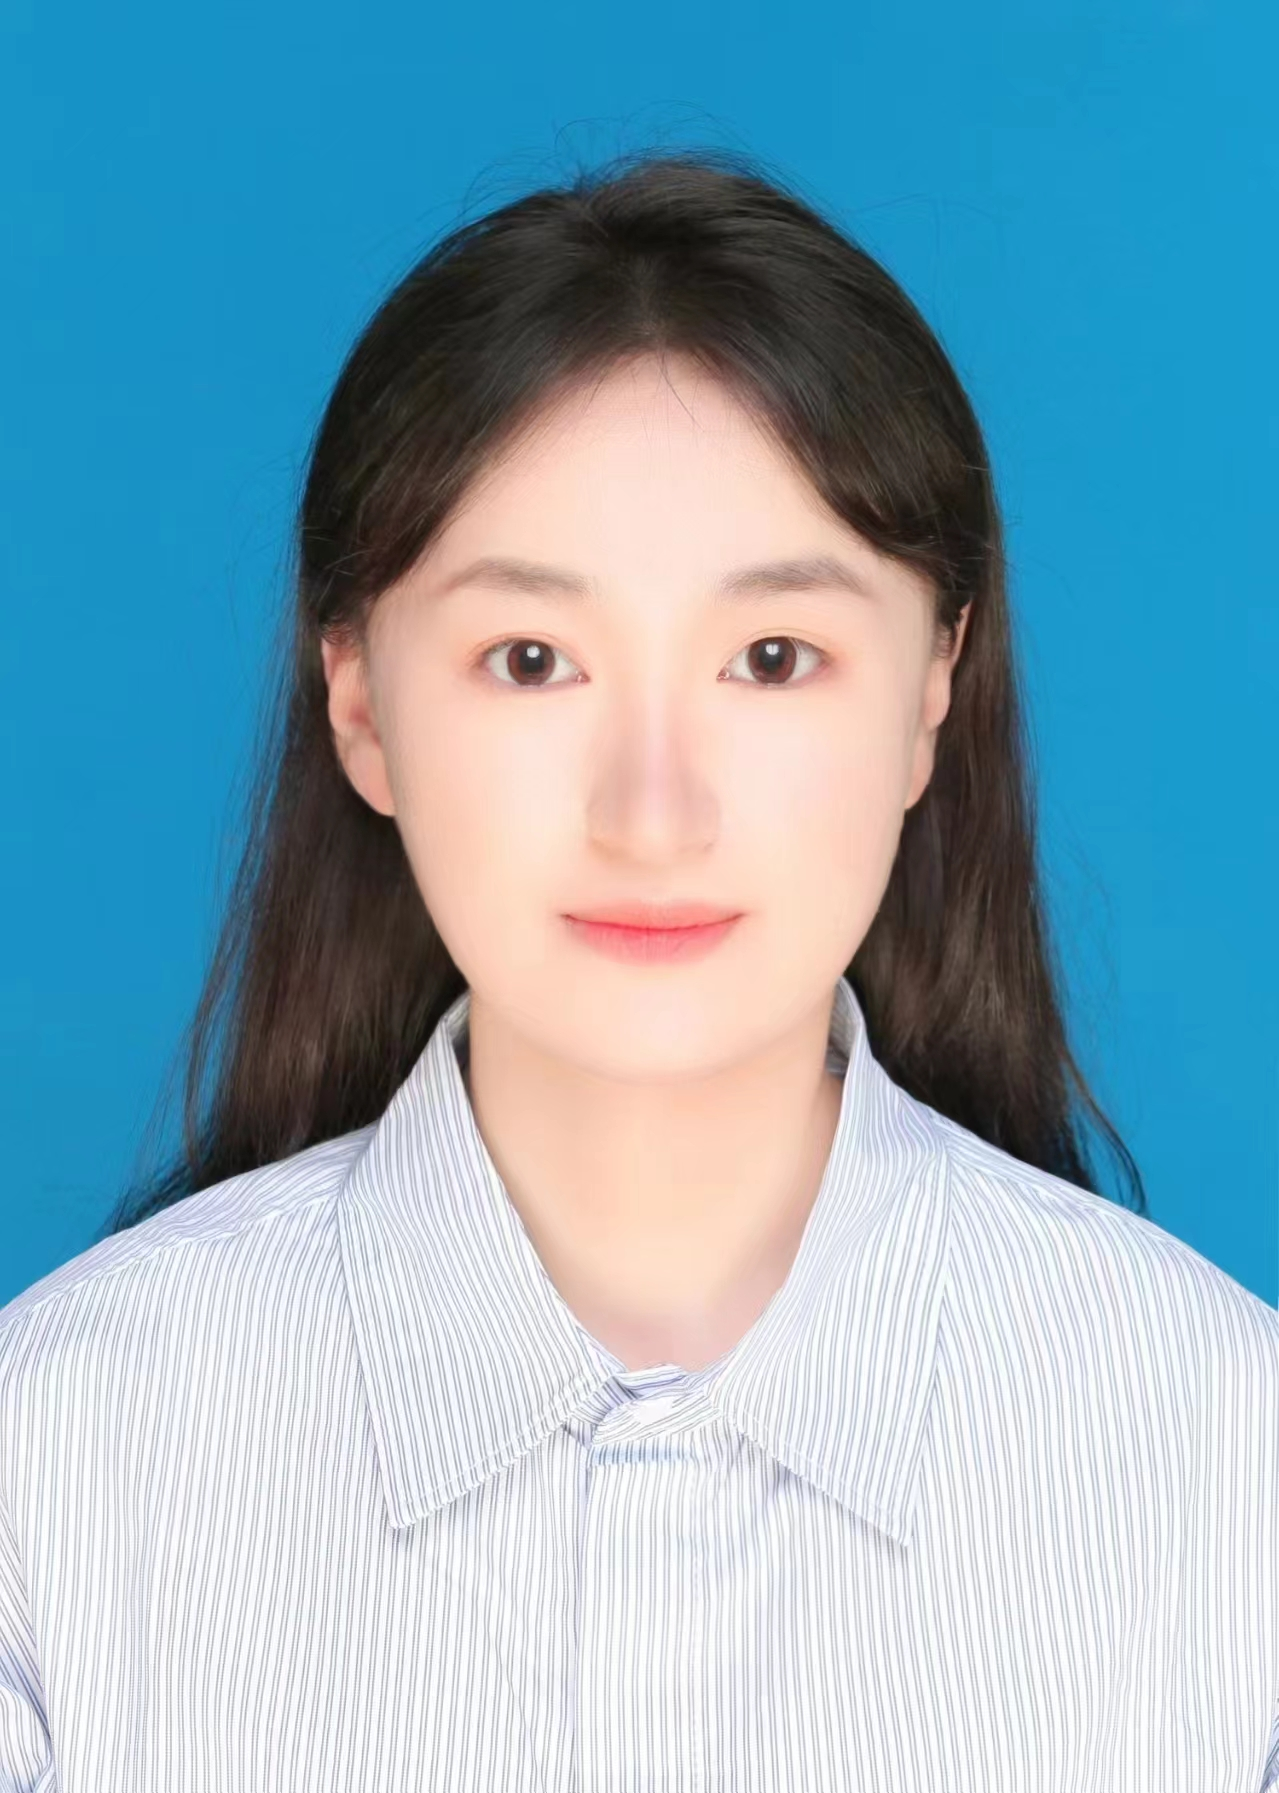
\includegraphics[height=3cm]{avatar.jpg}};
\end{tikzpicture}%
%%%% 利用tikz来定位学校Logo
\begin{tikzpicture}[remember picture, overlay] 
    \node[anchor = north west] at ($(current page.north west)+(1.2cm,-1.2cm)$) {
\includegraphics[height=1.2cm]{hit.jpg}};
\end{tikzpicture}%

% 姓名与联系方式（带定高盒子，完美避开照片并垂直居中）
\vspace*{-0.5em} 
\noindent
\begin{minipage}[c][3cm][c]{\textwidth - 3.5cm}
    \centering
    {\LARGE\bfseries{程昕蕊}}\\[0.4em]
     
    {\large \textbf{3D感知 / 世界模型 / Transformer / 端到端}}\\[0.5em]
    
    {\normalsize 
        女 $\vert$ 24岁 \quad
        \faPhone\ 150-4336-5908 \quad 
        \faEnvelopeO\ \href{mailto:cxrxin0530@163.com}{cxrxin0530@163.com} \quad
        \faGithubSquare\ \href{https://github.com/anonymou98/UNOP}{github.com/anonymou98/UNOP}
    }
\end{minipage}

% --- 在这里使用负间距将下方的正文往上拉 ---
\vspace{-0.4cm} % <--- 修改这个数值！如果你觉得还是宽，可以改成 -1cm 或 -1.2cm
    
% ================================================================
% 教育背景 ★差异：研究方向描述不同
% ================================================================
\section{\makebox[\widthof{\faGraduationCap}][c]{\color{CVBlue}\faGraduationCap}\ 教育背景} 

\textbf{哈尔滨工业大学} \quad 软件工程（电子信息） \quad 硕士研究生 \hfill 2024.9 -- 至今\\[0.2em]
\textcolor{CVBlue}{\textbf{排名：前20\%}} \quad \textbf{荣誉：}获得校级一等、二等学业奖学金

\textbf{长春工业大学} \quad 软件工程 \quad 本科 \hfill 2019.9 -- 2023.6\\[0.2em]
\textcolor{CVBlue}{\textbf{排名：前5\%}} \quad \textbf{荣誉：}在校期间获校级学业二等、三等奖学金共\textbf{6次}


% ================================================================
% ★★★ 改动2：新增「前沿论文复现」专节 —— 直击JD核心要求 ★★★
% ================================================================
\section{\makebox[\widthof{\faBook}][c]{\color{CVBlue}\faBook}\ 
前沿算法复现与跟踪}

\textbf{系统性复现多篇 Transformer-based 3D 
预测架构}（均基于车辆3D几何场景）
\hfill 2024.9 -- 至今
\begin{itemize}
    \item \textbf{Transolver}系列
    (ICML 2024)：基于Physics-Aware 
    Slice Attention的PDE求解器，
    复现并分析其在不规则网格上的
    注意力稀疏化策略。
    \item \textbf{GNOT}
    (ICML 2023)：General Neural 
    Operator Transformer，复现其
    异构输入编码与cross-attention
    多分辨率融合机制。
    \item \textbf{GAOT}
    (NeurIPS 2024)：Geometry-Aware 
    Operator Transformer，复现其
    几何编码与物理场耦合的注意力
    架构。
    \item 此外跟踪复现 \textbf{FNO / 
    Geo-FNO / PINO / GINO} 等
    神经算子方法，覆盖频域、
    图域、积分域三类范式。
    \item \textbf{所有模型均在车辆3D
    外流场数据集（ShapeNet-Car）上
    完成端到端训练与评估}，
    积累了丰富的\textbf{3D点云/网格
    数据处理、大规模模型训练调优}
    经验。
\end{itemize}


% ================================================================
% 科研经历
% ================================================================
\section{\makebox[\widthof{\faUsers}][c]{\color{CVBlue}\faUsers}\ 
科研经历}

% --- 科研一：UNOP ---
\textbf{UNOP：面向3D场景的长时物理世界模型} 
\textit{(一作，投稿至CCF-A)} 
\hfill 2025.3 -- 至今
\begin{itemize}
    \item \textbf{问题：}现有场景预测模型
    依赖大量标注数据，且自回归推理
    20步即发散，无法支撑长时序
    场景演化预测——这与自动驾驶中
    \textbf{世界模型需长时预测未来场景}
    的挑战高度一致。
    
    \item 提出基于\textbf{积分一致性}的
    无监督物理约束(LIPE)，
    \textbf{无需标注数据}即可训练，
    3D场景建模内存降至微分方法的
    \textbf{1/6}。
    
    \item 设计\textbf{几何解耦编码器(GALA)}
    统一处理不规则3D几何；
    \textbf{曲率感知门控(GSEO)}
    保留高梯度结构特征（类似
    自动驾驶中的边缘/遮挡区域）。
    
    \item \textbf{结果：}3D ShapeNet-Car 
    误差\textbf{4.06\%}，1D2D
    \textbf{50步长时外推仍稳定}
    （SOTA方法约20步发散），
    证明了长时序场景预测的
    可行性。
\end{itemize}

% ================================================================
% ★★★ 改动4：项目经历——重新包装叙事角度 ★★★
% ================================================================
\section{\makebox[\widthof{\faBriefcase}][c]{\color{CVBlue}%
\faBriefcase}\ 项目经历}

% --- 项目一 ---
\textbf{工业级3D数字孪生仿真系统
（端到端：数据→模型→部署）} 
\textit{(核心开发者)} \hfill 2024.12 -- 2025.6
\\[0.2em]
\textcolor{CVBlue}{\textbf{十四五国家重点研发计划项目}}
\begin{itemize}
    \item \textbf{3D数据Pipeline构建：}
    从零构建跨工具链数据流水线
    （3D几何清洗→坐标对齐→
    跨网格插值），处理\textbf{非结构化
    3D点云/网格}数据，经验可直接
    迁移至自动驾驶3D感知数据处理。
    
    \item \textbf{跨域迁移学习：}
    将汽车外流场AI模型\textbf{零样本
    跨域迁移}至水轮机内流场，
    模型架构不变即成功泛化，
    验证了3D几何表征的通用性。
    
    \item \textbf{虚实闭环系统：}
    设计``AI仿真基线+IoT实测''
    虚实对齐预警方案
    （类似自动驾驶\textbf{闭环仿真}
    思路），替代固定阈值规则，
    实现早期异常捕获。
    
    \item \textbf{成果：}推理\textbf{20ms}
    （加速$10^5\times$），
    课题\textbf{结题验收通过}，
    获3项发明专利+2项软著。
\end{itemize}

\projectsep

% --- 项目二 ---
\textbf{GeoGatedAttention：几何感知的
3D注意力机制设计} 
\textit{(核心开发者，发明专利已受理)} 
\hfill 2024.9 -- 2025.3
\begin{itemize}
    \item \textbf{动机：}标准Attention
    不感知3D边的几何结构，
    在几何突变区域（类似自动驾驶中
    车辆边缘/障碍物轮廓）
    预测误差大。
    
    \item 设计\textbf{几何门控注意力}
    (GeoGatedAttention)，
    用\textbf{边级几何特征动态调制
    attention权重}，实现
    \textbf{O(E)稀疏计算}——
    该机制可直接应用于
    BEV/3D检测中的几何感知模块。
    
    \item \textbf{结果：}预测误差
    \textbf{2.69\%}，相关系数
    $\rho$=\textbf{0.97}，
    推理\textbf{20ms}。
\end{itemize}








% ========================================================
\section{%
    \makebox[\widthof{\faTrophy}][c]%
    {\color{CVBlue}\faTrophy}\ 成果与获奖%
}

\begin{itemize}
    \item \textbf{学术论文：}Physics-Constrained Unsupervised Neural Operator for Long-Horizon PDE Learning on Generalized Geometries (\textbf{一作}，IJCAI CCF-A 审稿中)
    \item \textbf{专利：}一种结合几何特征与傅里叶神经算子的涡轮零件弹性数字孪生虚实交互方法 \textit{（实审中）}
    \item \textbf{专利：}基于几何门控注意力机制的结构感知图神经网络物理场预测方法 \textit{（实审中）}
    \item \textbf{专利：}一种基于应力驱动转速响应的水轮机风扇智能运维方法 \textit{（已公开）}
    \item \textbf{软件著作权：}多传感融合的部门数字孪生协同运维平台 (登记号: 2026SR0202932)
    \item \textbf{软件著作权：}设计-仿真部门数字孪生协同运维平台 (登记号: 2026SR0202550)
    \item \textbf{竞赛：}第十五届\textbf{中兴捧月}全球精英挑战赛 -- \textbf{区域优胜奖} \hfill 2025
\end{itemize}

  
% ================================================================
% 核心技能
% ================================================================
\section{\makebox[\widthof{\faCogs}][c]
{\color{CVBlue}\faCogs}\ 核心技能}
    
\begin{itemize}
    \item \textbf{深度学习架构：}
    深入理解\textbf{Transformer}架构
    （Self/Cross-Attention、
    稀疏注意力、几何感知注意力）；
    熟悉\textbf{GNN/图神经网络}
    在3D场景中的应用；
    了解\textbf{Diffusion Model}
    基本原理。
    
    \item \textbf{3D视觉与感知：}
    熟练处理\textbf{3D点云、
    非结构化网格}数据；
    熟悉VTK/ParaView 3D可视化；
    了解\textbf{BEV感知、NeRF、
    3D Gaussian Splatting}
    基本原理。
    
    \item \textbf{模型训练与调优：}
    熟练使用\textbf{PyTorch / PyG}；
    有大规模3D模型训练、
    长时序自回归预测、
    多GPU训练经验。
    
    \item \textbf{工程能力：}
    Python, C++(基础), 
    Linux, Docker, Git；
    代码风格良好，
    熟悉模块化开发。
    
    \item \textbf{论文能力：}
    持续跟踪\textbf{CVPR/NeurIPS/
    ICML/ICLR}等顶会论文，
    已独立复现\textbf{10+篇}
    前沿工作；CET-6通过。
\end{itemize}

% ================================================================
% 个人评价
% ================================================================
\section{\makebox[\widthof{\faUser}][c]
{\color{CVBlue}\faUser}\ 个人评价}

\begin{itemize}
    \item \textbf{3D场景理解能力突出：}
    深耕3D几何编码与物理场预测，
    对\textbf{不规则几何的
    Transformer建模}有深入理解，
    可快速迁移至自动驾驶
    3D感知/BEV/世界模型方向。
    
    \item \textbf{强论文复现与创新能力：}
    系统复现GNOT/GAOT/Transolver等
    10+篇顶会工作，并在此基础上
    提出创新方法投稿CCF-A。
    
    \item \textbf{端到端落地经验：}
    从数据pipeline构建、模型设计
    训练到工程部署，
    完整交付国家级项目。
\end{itemize}
\end{document}
